\documentclass[12pt]{report}

%math packages
\usepackage{amssymb}
\usepackage{amsmath}
\usepackage{amstext}
\usepackage{dsfont}

%other packages
\usepackage{natbib}
\usepackage{comment}
\usepackage{graphicx}
\usepackage{float}
\usepackage{epstopdf}
\usepackage[pdftex,colorlinks]{hyperref}
  \hypersetup{linkcolor=black,urlcolor=black,citecolor=black}


%page setup
\usepackage{geometry}
\geometry{letterpaper}
\usepackage{fullpage}

\title{User Guide\\ \vspace{0.1in} \large{Curvilinear Navier-Stokes (CNS) C++ Code}}
\author{Bobby Arthur \\ Department of Civil and Environmental Engineering
                     \\ Environmental Fluid Mechanics Laboratory
                     \\ Stanford University}
\date{\today}

\begin{document}
\maketitle
\tableofcontents

\chapter{Code Structure}

\section{Introduction}
This curvilinear Navier-Stokes (CNS) C++ code is also known as ``cns-koltakov" or, more affectionately, ``Sergey's Code," after its author, Sergey Koltakov. It is the third version of the original Fortran code written by Yan Zang at Stanford in the early 1990's \citep{zang1994}. The original code was serial (one processor). The second version was updated by Cui to run with multiple processors using MPI, and is known as PCUI \citep{cui2001}. This latest version of the code is basically a translation of PCUI to C++ using an object-oriented framework, which allowed for the addition of a moving grid \citep{koltakov2012}. Over the years, these various versions of the code have been used to study a wide range of geophysical flows.

The code is based on the fractional step method of \citet{zang1994} and includes the LES model of \citet{zang1993}. It solves the incompressible Navier-Stokes equations on a generalized curvilinear grid with a rigid lid, employing a semi-implicit time integration scheme with Adams-Bashforth for the explicit terms and Crank-Nicholson for the implicit terms. Additionally, it uses the QUICK and SHARP schemes for advection of momentum and scalars, respectively, and solves the pressure Poisson equation with a multigrid method. 

\section{File Summary}
The code is contained in the directory \texttt{/cns-koltakov}, which contains the following files:
\begin{description}
\item[\texttt{Makefile}] \hfill \\Used to compile and run the code (see \hyperref[sec:start]{Section \ref*{sec:start}}).
\item[\texttt{parameters.dat}] \hfill \\The main input file for the code, which contains the most commonly adjusted variables. The file is read at runtime, so the user may redefine variables without recompiling the code.
\item[\texttt{parameters.h}] \hfill \\Defines all the parameters for the code, including physical variables, boundary conditions, and multigrid parameters. Also allows the user to turn different modules (e.g. scalar advection, moving grid, etc.) on or off, run predefined cases (see \hyperref[chap:examples]{Chapter \ref*{chap:examples}}), or change the bottom bathymetry. In order to modify \texttt{parameters.dat}, the function \texttt{Set\_Parsable\_Values()} must be modified here.
\item[\texttt{test.cpp}] \hfill \\The main loop of the code. 
\item[\texttt{navier\_stokes\_solver.h}/\texttt{.cpp}] \hfill \\Contains the time-stepping scheme for the momentum equations, including, most importantly, the \texttt{Predictor()} and \texttt{Corrector()} schemes. Also where all arrays containing physical variables are initialized. Additionally, the scalar solve, background potential energy, post-processing, and other similar functions are called here.
\item[\texttt{pressure.h}] \hfill \\Contains the multigrid pressure Poisson equation solver.
\item[\texttt{scalar.h}] \hfill \\Updates scalar quantities after the velocity has been updated.
\item[\texttt{convection.h}] \hfill \\Contains the advection schemes used in the code, specifically, QUICK for momentum advection and SHARP for scalar advection.
\item[\texttt{universal\_limiter.h}] \hfill \\Contains the limiter used in the above advection schemes.
\item[\texttt{tridiagonal\_solver.h}] \hfill \\Contains functions used to solve tridiagonal systems with periodic or non-periodic boundary conditions. Used both in the implicit part of the momentum and scalar solutions, as well as the smoothing operation in the multigrid solver.
\item[\texttt{curvilinear\_grid.h}/\texttt{.cpp}] \hfill \\Creates the grid and calculates the necessary metric quantities. Note that a custom grid (stored as a binary file) can be used if \texttt{read\_grid\_from\_file} is set to \texttt{true} and \texttt{grid\_filename} is specified in \texttt{parameters.h}.
\item[\texttt{mpi\_driver.h}/\texttt{.cpp}] \hfill \\Initializes and controls parallel implementation using MPI. Also defines binary output functions.
\item[\texttt{metric\_quantities.h}] \hfill \\Defines the metric quantities that are calculated in \texttt{curvilinear\_grid.cpp}.
\item[\texttt{array\_Xd.h}/\texttt{.cpp}] \hfill \\Classes that define all array operations in the code, where \texttt{X} is a number 1-3.
\item[\texttt{potential\_energy.h}] \hfill \\Calculates the background potential energy and related quantities. Note that kinetic energy and dissipation are calculated in \texttt{navier\_stokes\_solver.cpp}.
\item[\texttt{turbulence.h}] \hfill \\Contains the turbulence model, which is not fully implemented (yet).
\item[\texttt{curvilinear\_moving\_grid.h}/\texttt{moving\_grid\_engine.h}] \hfill \\Implementation of the moving grid.
\item[\texttt{interpolant.h}] \hfill \\Used with the moving grid to interpolate physical variables from the old to new grid.
\item[\texttt{data\_aggregator.h}] \hfill \\Aggregates time-series of physical variables.
\item[\texttt{parameter\_file\_parser.h}] \hfill \\Reads the input file \texttt{parameters.dat}.
\end{description}

\section{Getting Started}\label{sec:start}
To begin using the code, it must first be compiled with the Intel C++ Compiler (\texttt{icc}) and the MPICH compiler (\texttt{mpicc}). A free version of the Intel C++ Compiler can be found at \url{http://software.intel.com/en-us/non-commercial-software-development}, while MPCIH can be found at \url{http://www.mpich.org/downloads/}. Note that MPICH must be compiled on your machine with the Intel compiler \texttt{icc} flag, see the MPICH documentation for specifics.

Once the compilers have been downloaded, make sure that the path to \texttt{mpicc} is specified correctly in the Makefile next to \texttt{CC=}. Then, the code can be compiled with \texttt{make test} and run with \texttt{make runX}, where \texttt{X} is the number of processors. Note that this number must agree with what is specified in \texttt{parameters.dat}. That is, \texttt{X = num\_cpu\_x*num\_cpu\_y*num\_cpu\_z}.

 
\chapter{Code Output}

\section{Binary Output}
The code output is contained in binary files that correspond to a specific processor. 
Data is output for the variables specified in \texttt{parameters.h} at the frequency 
defined by \texttt{save\_timestep\_period} in \texttt{parameters.dat}. These files will be stored in \texttt{output\_dir} defined in \texttt{parameters.dat}. The files are organized by variable and processor. For example, the velocity output from the 0th processor will be stored in \texttt{velocity.0}.

\section{Loading and Viewing Output Data}
The \texttt{/cns-koltakov/mfiles} directory contains MATLAB scripts to view data from binary output directly, or to load \texttt{.mat} files which can be used in your own scripts. The files included in this directory are as follows.

\begin{description}
\item[\texttt{cns\_viz.m}] \hfill \\Plots 2D slices of any physical variable or 3D isosurfaces of density and vorticity.
\item[\texttt{cns\_load.m}] \hfill \\Loads physical variables into matrices that are stored in a \texttt{.mat} file.
\item[\texttt{cns\_load\_energy.m}] \hfill \\Loads a time series of energy quantities and saves a \texttt{.mat} file.
\item[\texttt{load\_binary\_X.m}] \hfill \\Functions that load data directly from binary output files and return a 3D (x,y,z) matrix.
\item[\texttt{calculate\_binary\_X.m}] \hfill \\Functions that calculate other quantities (e.g. vorticity) using data from binary output files.
\end{description}

\section{Restarts}
The code is able to save data for restarts if a nonzero value for \texttt{restart\_timestep\_period} is given in \texttt{parameters.dat}. This will save restart files at the specified period named \texttt{restart\_tX.0}, where \texttt{X} is the time step. To run a restart job, specify \texttt{restart\_timestep} and \texttt{restart\_dir} (where the restart files from the old run were stored) in \texttt{parameters.dat}. Make sure to change \texttt{output\_dir} so that your old data is not overwritten. Then, run the job as usual with \texttt{make runX}. Note that \texttt{max\_timestep} still starts from 0, not from the restart timestep.

\chapter{Examples}\label{chap:examples}
The following example cases have been set up in the code. Going through them provides a good introduction to different parameters and variables, as well as how to view output using \texttt{cns\_viz.m}. 

\section{Internal Seiche}
To run the internal seiche test case, set \texttt{internal\_seiche} to \texttt{true} in \texttt{parameters.h}. This will initialize the density field with
\begin{equation}
\frac{\rho}{\rho_0}=1-\frac{\Delta\rho}{2\rho_0}\text{tanh}\left(\frac{2(z+H/2-a\text{cos}(\frac{2\pi}{\lambda}x)}{\delta}\text{tanh}^{-1}(\alpha)\right),
\end{equation}
as shown in \hyperref[fig:seiche]{Figure \ref*{fig:seiche}}. Try running this case with a domain size of 1$\times$0.25$\times$1 m and a grid of size 32$\times$8$\times$32 and a time step of 0.1 s. 
\begin{figure}
\centering
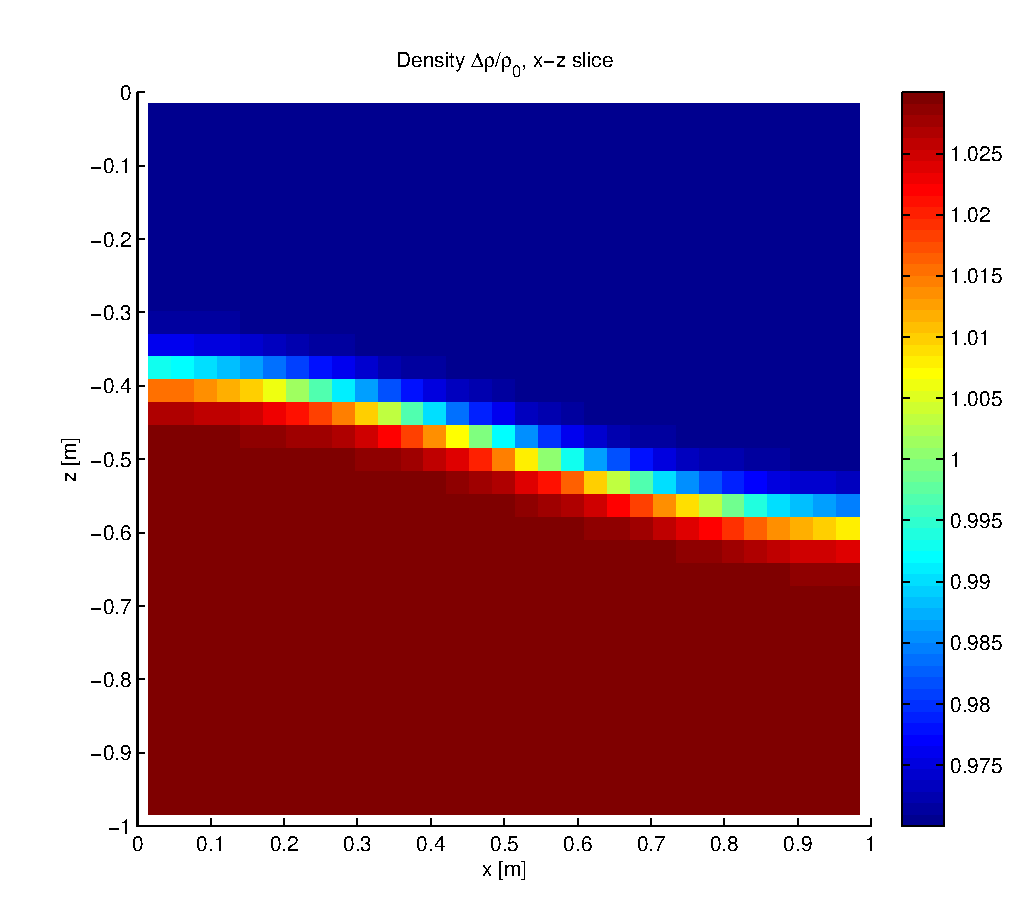
\includegraphics[scale=0.6]{seiche}
\caption{Initial density profile for internal seiche case, plotted using \texttt{cns\_viz.m}.}
\label{fig:seiche}
\end{figure}

\section{Lid-driven Cavity}
To run the lid-driven cavity test case, set \texttt{lid\_driven\_cavity} to \texttt{true}  
and \texttt{scalar\_advection} to \texttt{false} in \texttt{parameters.h}. This will initialize a horizontal velocity $u=0.1$ m/s on the top of the domain. Also set
\texttt{molecular\_viscosity} to $10^{-3}$ m$^2$/s in \texttt{parameters.dat}. Over time, circulation will develop in the domain. Try running this case with a domain size of 1$\times$0.25$\times$1 m (giving $Re=uL/\nu=100$), a grid of size 32$\times$8$\times$32, and a time step of 0.1 s. After 300 time steps, or 30 s, the flow should look like \hyperref[fig:lid]{Figure \ref*{fig:lid}}. 
\begin{figure}
\centering
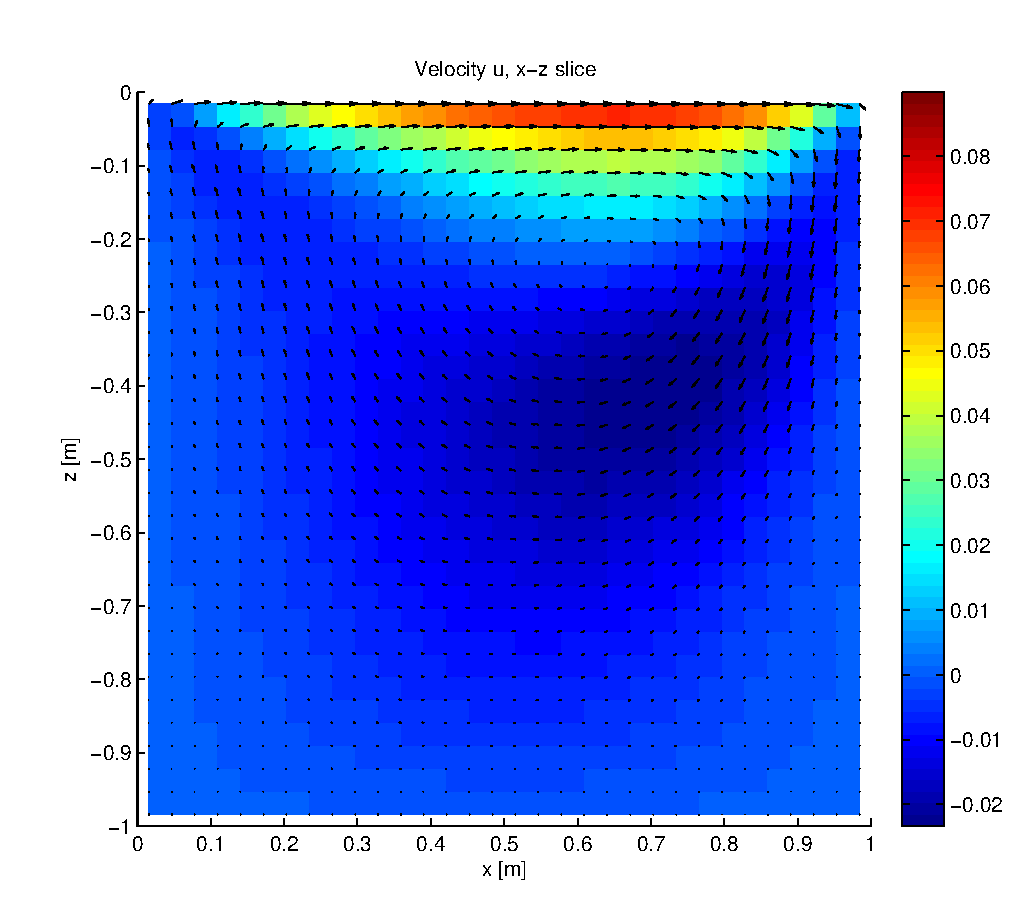
\includegraphics[scale=0.6]{lid}
\caption{Horizontal velocity with velocity vectors for lid-driven cavity case after 300 time steps, or 30 s, plotted using \texttt{cns\_viz.m}.}
\label{fig:lid}
\end{figure}

\section{Lock Exchange}
To run the lock exchange test case, set \texttt{lock\_exchange} to \texttt{true} in \texttt{parameters.h}, and make sure \texttt{scalar\_advection} is set back to \texttt{true}. The domain will be initialized with dense fluid on the left side and heavy fluid on the right. Over time, density currents will develop and propagate in both directions. Try running this case with a domain size of 4$\times$0.25$\times$0.5 m, a grid of size 128$\times$8$\times$16, $\nu=10^{-6}$ m$^2$/s, a time step of 0.1 s, and a free-slip bottom boundary condition. After 800 time steps, or 80 s, the flow should look like \hyperref[fig:lock]{Figure \ref*{fig:lock}}. 
\begin{figure}
\centering
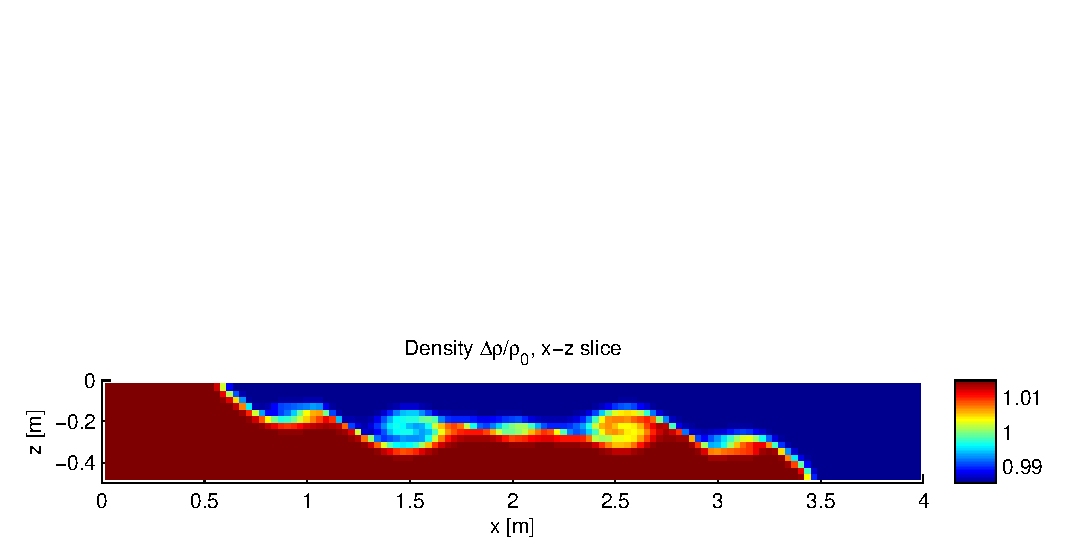
\includegraphics[scale=0.9]{lock}
\caption{Density structure of lock exchange after 800 time steps, or 80 s, plotted using \texttt{cns\_viz.m}.}
\label{fig:lock}
\end{figure}
Check out the shear instabilities that develop at the interface!

\section{Breaking Internal Wave}
Two types of internal wave cases can be run in the code: solitary waves and progressive waves. To run a solitary wave, set \texttt{solitary\_wave} to \texttt{true} in \texttt{parameters.h}. To run a progressive wave, set \texttt{progressive\_wave} to \texttt{true} in \texttt{parameters.h}. For both cases, set \texttt{variable\_fixed\_depth} to \texttt{true} in \texttt{parameters.h}, and specify the start of the slope \texttt{x\_s}, the slope value \texttt{slope}, and the interface depth ($h_1$) \texttt{upper\_layer\_depth} in \texttt{parameters.dat}. Try running both cases with a domain size of 3$\times$0.25$\times$0.5 m, a grid of size 512$\times$16$\times$32, $\nu=10^{-6}$ m$^2$/s, a time step of 0.01 s, and a no-slip bottom boundary condition. Set the slope to start at $x=1$ m and the slope itself to be 0.218. Also specify $\alpha=0.99$, $\delta=0.1$ m, $\Delta\rho/\rho_0=0.03$, $\rho_0=1000$ kg/m$^3$, and $h_1=0.3$ m.There are additional parameters for each case that can be specified in \texttt{parameters.dat}. For the solitary wave, set the amplitude \texttt{a} to 0.1 m and the wavelength \texttt{Lw} to 0.7 m. For the progressive wave, set \texttt{forcing\_amp} to 0.05 and \texttt{forcing\_period} to 10 s. 

Note that the solitary wave case uses closed boundaries, and is created by an initial gaussian in the interface on the left (west) side of the domain. The progressive case, however, uses an open boundary condition, where the horizontal velocity \texttt{u(i,j,k).x} and horizontal volume flux \texttt{U\_xi} are specified on the west boundary. These fluxes must conserve volume in the domain by having a net zero flow. Look at \texttt{Set\_Progressive\_Wave\_BC()} in \texttt{navier\_stokes\_solver.cpp} and \texttt{Quick\_Velocity\_Flux\_Update()} in \texttt{convection.h} to see how this boundary condition is implemented.

The initial condition for the solitary wave run can be see in \hyperref[fig:solitary]{Figure \ref*{fig:solitary}}, while \hyperref[fig:solitary]{Figure \ref*{fig:solitary}} shows a progressive wave after X time steps, or X s. Run each case yourself to see the wave breaking on the slope! Note that this example has a much larger grid size than the previous examples; you will need to use multiple processors to get a reasonable runtime.
\begin{figure}
\centering
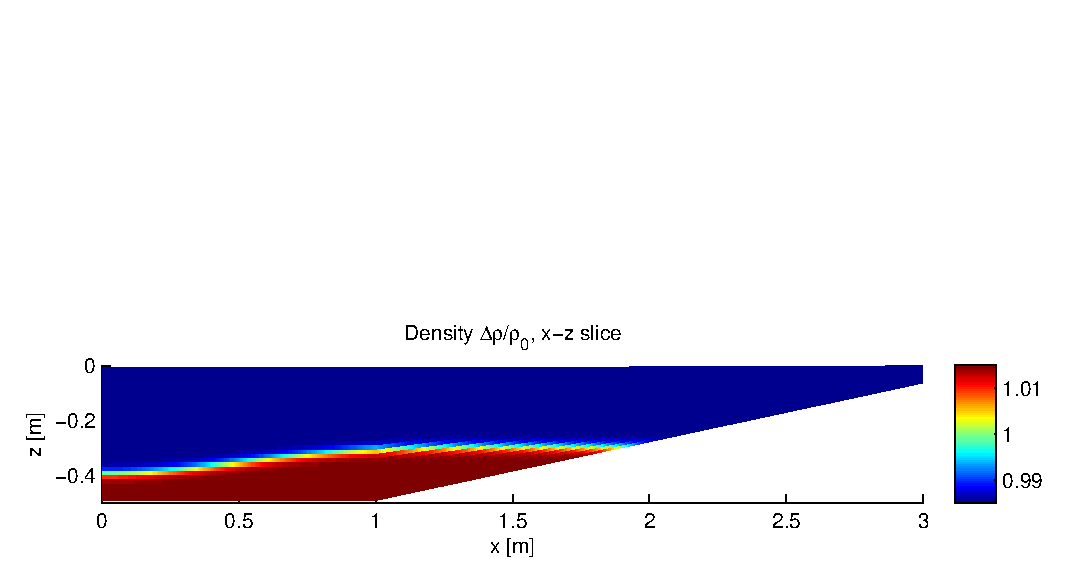
\includegraphics[scale=0.9]{solitary}
\caption{Initial density profile of solitary wave case, plotted using \texttt{cns\_viz.m}.}
\label{fig:solitary}
\end{figure}

\section{Sediment Transport}
Coming soon!

\bibliographystyle{apalike}
\bibliography{cns_user_guide}

\end{document}
